\documentclass[a4paper,10pt]{article}

\usepackage{fancyhdr} % clears the header and footer setting
\usepackage{graphicx} 
\usepackage{geometry}
\geometry{a4paper, left=2cm, right=2cm, top=1.5cm, bottom=3cm }
\usepackage{caption}
\usepackage{subcaption}
\usepackage{hyperref}
\usepackage{natbib}

\usepackage{etoolbox,fancyhdr,xcolor}
\newcommand{\headrulecolor}[1]{\patchcmd{\headrule}{\hrule}{\color{#1}\hrule}{}{}}
\newcommand{\footrulecolor}[1]{\patchcmd{\footrule}{\hrule}{\color{#1}\hrule}{}{}}
\renewcommand{\headrulewidth}{1pt}
\headrulecolor{red!100}%
\renewcommand{\footrulewidth}{1pt}
\footrulecolor{red!100}%

\fancyhf{}
\fancyhead[R]{
\includegraphics[width=0.25\textwidth]{nmims.png}}

\fancyfoot[C]{Nilkamal School of Mathematics, Applied Statistics & Analytics}
\fancyfoot[R]{\thepage}

\setlength{\headheight}{15mm}
\pagestyle{fancy} %This command sets the page style to fancy, applying the header and footer configurations defined above to the document pages.

\bibliographystyle{apacite}

\usepackage{times}
\begin{document}

\noindent 
\begin{center}
\textbf{{\Large Role of Green Packaging In Consumer Purchasing Decisions using Logistic Regression}} \\
\end{center}

\noindent 
\textbf{Nitya Verma,} \textit{Narsee Monjee Institute Of Management Studies, Mumbai}\\

\noindent 
\textbf{ABSTRACT: } The abstract is a summary of your research project and includes motivation, aims, methods used, (preliminary) findings and (preliminary) conclusions.  The abstract should be a stand-alone document that someone could read to get a general overview of your research project.  

Write the abstract the font shown but make sure it is no longer than about 500 words (and it must fit on a single page which includes the title, authors and keywords). The words of ‘Abstract’ and ‘Keywords’ are set in bold and full caps.  Make sure you put your correct project code in the footer. If you have two supervisors you can list both of them.  If one of them is from industry you should give their company name etc.
Please note the following rules regarding the final paper:
\begin{itemize}
    \item First page (starts with - Title, Authors, Abstract(s) and Keywords) [MANDATORY] and then follows
    \item Body of the paper (text and tables and or figures in the format shown) [MANDATORY]
    \item Notation [OPTIONAL]
    \item Appendices [OPTIONAL]
    \item References [MANDATORY]
\end{itemize}

The total length of the paper is to be no more than \textbf{14pp for 3rdyr and 19pp for 4thyr}. A cover sheet is also required in addition to the research paper. Note that the cover sheet is not included in the page limit.
\\

\noindent 
\textbf{KEYWORDS:} Keyword 1, Keyword 2 and Keyword 3. You can include a maximum of 6 keywords for indexing purposes (spaced by commas). Keywords are single words or short phrases describing the main concepts/topics covered in the paper. Sometimes only 2 or 3 keywords will suffice, but definitely no more than six.\\


\section{INTRODUCTION}

Consumers are the essence of any business. They come at the top of the development process of every business.\cite{Witek2020}. The phrase customer is king is valid in every venture across the globe as they make or break a business. The importance given to the customers makes it all the more crucial to understand their psyche and behaviour as that directly impacts the firms' profit and longevity. 

Corporate Social Responsibility (CSR) activities were made mandatory in April 2014 under the Companies Act 2013. The main aim of this modification by the Government of India was to inculcate a sense of social consciousness in the firms. The increase in environmental degradation made it all the more vital for the firms to make small changes to influence society at large, which led to the popularity of a new term known as "Green Marketing". Green Marketing came into emergence in the 1980s. It simply means the promotion, distribution, and packaging of products and services by focusing on their sustainability and ecological benefits. 
It's no surprise that environmental contamination is at its peak currently \cite{RaviVyas2023}. An enormous bulk of this contamination comes from waste packaging. 

\subsection{Secondary Heading or Sub-headings}

Here we have a sub-heading. There is no blank line after the sub-heading. You can have one level of subheadings but not a third i.e. you cannot have Section 1.1.1 as a subheading.

\begin{itemize}
    \item If you want to list bullet points you can do so;
    \item This is the second point;
    \item This is a third bullet point;
    \item A fourth bullet point;
    \item But you can.
\end{itemize}   

After a list you must leave a single blank line and remember to add the indent if you are starting a new paragraph.

\subsection{Another sub-heading}

You can have as many sub-headings in a section as you want to. Note that sub-headings have a 6pt spacing after them rather than a blank line but they are preceded by a blank line. The number of sections and sub-sections is up to you, as are the titles of each of them and this will be driven by the content of your report.

\section{NEW SECTION}

\subsection{How to make citations?}

We want you to use the Harvard referencing system so let’s try it out. \cite{Witek2020} provide a  systematic review of existing approaches of sensitivity analysis of environmental models. If you want to quote from a source directly please make sure you enclose the words as follows. \cite{norman2006} state that “our integrated approach to research has enabled us to design, construct and accurately control the first dedicated multiple support excitation experimental test bed.”.   \cite{smith2006} explain how “experimental research is also enabling us to validate numerical methods through comparison of results with experimental tests”. \cite{norman2006} give the following description of BLADE: 

“…with the recent opening of BLADE (Bristol laboratories for advanced dynamic engineering) the scope for real time large scale testing has greatly increased. Our integrated approach to research has enabled us to design, construct and accurately control the first dedicated multiple support excitation experimental test bed for testing scale models of long span bridges. This test bed is being used to help increase our understanding of the effects of MSE on structures.”

There are other ways to make citations, for instance when you have not mentioned the name of the author in your sentence. This citation is generally placed after the relevant quote or paraphrase, or at the end of the sentence. See the following examples. Environmental modelling is used for process understanding and for prediction for practical applications \citep{beven2018}.  Nitrogen concentrations in the Thames catchment have increased since 1930 due to land management practices \citep{howden2011}. Multiple citations can be included at the end of a sentence or paragraph \citep{beven2018, howden2011}. 

The general rule is do not copy-paste material from other papers. Always write the material with your own words and make the appropriate citations. Use paraphrasing, summarising and quoting when citing other sources.  See also the University advice on plagiarism at: \href{https://www.bristol.ac.uk/students/support/academic-advice/plagiarism/}{https://www.bristol.ac.uk/students/support/academic-advice/plagiarism/}.

You may use recognized abbreviations for journal titles e.g. Can. Geotech. J. for Canadian Geotechnical Journal. If you need to look up the journal title look up \href{http://cassi.cas.org/search.jsp}{http://cassi.cas.org/search.jsp} (accessed 5th March 2017). Only do this if you need to save space as the full title does make searching easier.

You can abbreviate journal/proceedings titles in the bibliography file (if needed to save space). Follow this \href{https://images.webofknowledge.com/images/help/WOS/A_abrvjt.html}{link}
with the correct abbreviations for journals from the web of science.



\subsection{How to include equations, figures and tables?}

Some of us like to include a formula or two and these should be referred to in the test in the form equation 1. You must type in equations using the equation editor and all symbols should be explained within the text of your manuscript. However you may prefer to include a separate section detailing all nomenclature. Never paste equations in from a paper or other source. Leave a blank line before and after the equation:

\begin{equation}
x = \frac{-b \pm \sqrt{b^2 - 4ac} }{2a}
\end{equation}

where $x$ is a number; $a$, $b$, and $c$ are other numbers.

\begin{equation}
BCP = 176R+28G+46B
\end{equation}

where, $BCP$, $R$, $G$ and $B$ are also useful numbers.

Figure \ref{fig_regression} shows a graph.  Figures / diagrams / photos are to be centred, with the reference and caption printed below the figure. The lettering used in the illustrations should be easily legible.  Illustrations are to be referred to as figures, and must be quoted in the text. One blank line should be left between the figure caption and the next paragraph. Please ensure that all figures are of the highest quality. Keep figures as simple as possible. Avoid excessive notes. Photographs must have a resolution of at least 300 dpi. The use of colour is allowed on figures. Note that the test does not wrap around the figure but if you do not like the wasted space then it is acceptable to put two figures side by side but they must be e.g. a ‘Figure \ref{fig_bridge1}’ and ‘Figure \ref{fig_bridge2}’ and not ‘Figure 1’ and ‘Figure 2’. See the example given as Figure \ref{fig_twobridges}. However all figures must be as close as possible to the location where they are first referred to in the text. The figure is also not surrounded by an unnecessary box/border. Remove this when inserting figures from MS Excel.


\begin{figure}[ht]
\centering
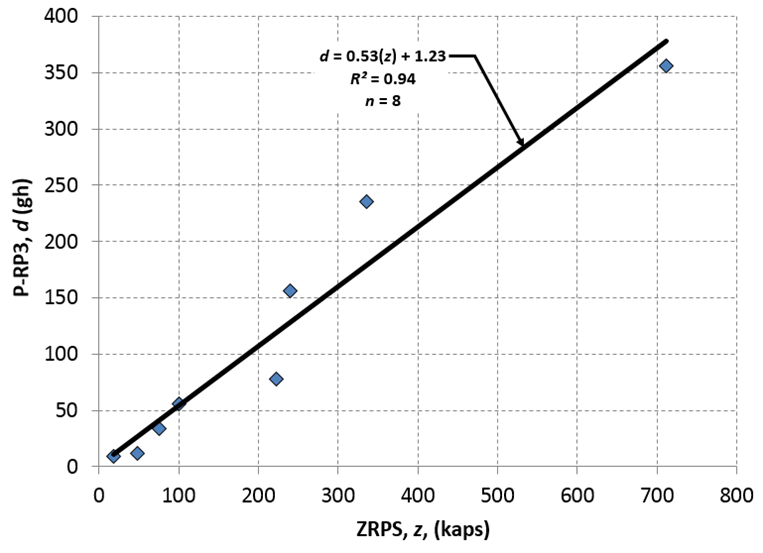
\includegraphics[height=6.6cm]{figures/fig_regression}
\caption{An interesting plot (note that figure captions go BELOW THE FIGURE).}
\label{fig_regression}
\end{figure}


\begin{figure}[ht]
     \centering
     \begin{subfigure}[b]{0.45\textwidth}
         \centering
         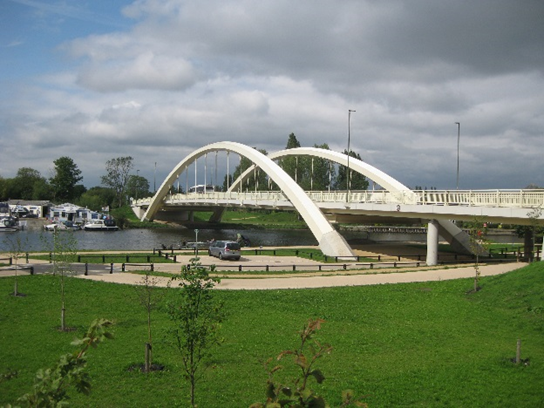
\includegraphics[width=\textwidth]{figures/fig_bridge1}
         \caption{Bridge 1}
         \label{fig_bridge1}
     \end{subfigure}
     \hfill
     \begin{subfigure}[b]{0.45\textwidth}
         \centering
         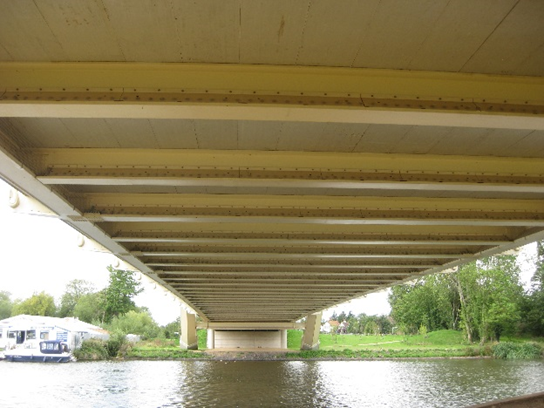
\includegraphics[width=\textwidth]{figures/fig_bridge2}
         \caption{Bridge 2}
         \label{fig_bridge2}
     \end{subfigure}
        \caption{Walton-on-Thames Bridge (a) wide shot and (b) the underside of the deck
(photos taken by P. J. Vardanega, used with permision)}
        \label{fig_twobridges}
\end{figure}



\section{NEXT HEADING}

Table \ref{tab_materials} contains something interesting. For tables make sure that you use 8 point Times New Roman for ALL the text in the Tables (apart from the caption). Please be consistent throughout your manuscript. Leave one blank line before the table title, another blank line after the title and one blank line after the table. Table titles must be above the table. As with figures the use of color is acceptable in tables. Make sure that the table does not run across multiple pages. If it does then have a repeat of the table caption with the word ‘continued’ in brackets after it.


\begin{table}[h]
\begin{center}
\caption{Summary of the database (note that table captions go ABOVE THE TABLE)}
\begin{tabular}{ |l|c|l| }
\hline
 \textbf{Column heading} & \textbf{Column heading}    & \textbf{Column heading} \\ \hline 
 Table Text     & 10     & Falling head permeameter \\  \hline 
 Concrete       & 2      & Strong \\ \hline 
 Steel          & 1      & Stronger \\ \hline 
 Timber         & 3      & Weak \\ 
 \hline
\end{tabular}
\label{tab_materials}
\end{center}
\end{table}


\section{SUMMARY}

The conclusions to be drawn from this work are as follows:
\begin{itemize}
    \item 	This is a great template
\end{itemize}


At the end of the reference list no more than 15 pages should be in your ENTIRE document (including the cover sheet). Do check else a penalty will be applied!  (For students enrolled in CENGM0080 your document including the cover sheet must be no longer than 20 pages using this template).

Remember you need to submit your research paper as a PDF document! Make sure you check that all the fonts, figures and text is preserved in the layout you intend when PDF conversion is done!


\subsection{Limitations and Recommendations for further work}

For this research paper it is useful to include this section where you discuss the limitations of your work and point to future work.

\section{ACKNOWLEDGEMENTS}

Use this section to thank people who have assisted during the project – if you want. It is good form to thank your supervisor, technicians and doctoral students who have helped and anyone else who deserves a mention – but do not make it too personal. 

For example, ‘the author wishes to thank Dr X for their supervision throughout the year and also Mr G who helped build the testing rig described in this paper.’
Use this section to thank your data sources including citations to the data, weblinks, etc.

\section{APPENDIX I}

These are NOT RECOMMENDED. However, if you want to put a mathematical derivation or large data table at the back of the paper in an appendix please put it before the NOTATION LIST. 

\section{APPENDIX II}

If a second appendix is used then call the first appendix ‘APPENDIX I’ and the second ‘APPENDIX II’ and so on.

\section{NOTATION}

This section is optional. If you have few equations it may be better to simply define all the variables in the text as shown. For highly mathematical papers this section is very helpful for the reader. Note that this section heading is not numbered. Please put the following statement in italics before the notation list:

\textit{The following acronyms and symbols are used in the work described in this paper:}

\textbf{Acronyms}

BSI	 British Standards Institute

\textbf{Symbols}

\textit{Latin}

$A$ = a constant

\textit{Greek}

$\gamma$ = shear strain



\fontsize{8}{9}\selectfont
\bibliography{ResearchPaperBib}



\clearpage



\end{document}